\question{2}{7} The number line represents elevations in metres relative to sea level.
\begin{center}
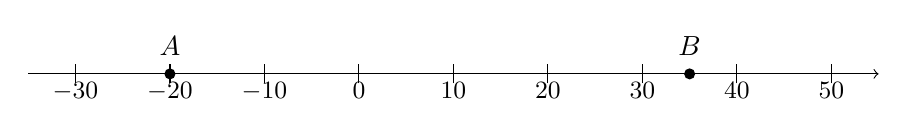
\begin{tikzpicture}[x=0.12cm,y=1cm]
  \draw[->] (-35,0)--(55,0);
  \foreach \x in {-30,-20,...,50} {\draw (\x,-0.12)--(\x,0.12) node[below=3pt] {\small $\x$};}
  \fill (-20,0) circle (2pt) node[above=3pt] {$A$};
  \fill (35,0) circle (2pt) node[above=3pt] {$B$};
\end{tikzpicture}
\end{center}
\begin{subparts}
  \item Write down the elevation of $A$ and the elevation of $B$.
  \item Which point is higher, and by how many metres?
  \item A drone is $18$ m below point $B$. Mark its elevation, $C$, on the number line and state whether $C$ is above or below sea level.
  \item A cave is lower than $A$ but higher than $-30$ m. Write down two possible integer elevations for the cave.
\end{subparts}
\answerlines{15}
